
\chapter{Алгоритмы оценки состояния}
\label{chapter_estimation}

Для реализации обратных связей в контуре управления необходимо обеспечить оценку текущего положения, скорости, кватерниона ориентации и угловой скорости БЛА. Получить данные оценки можно с помощью стандартного набора бортовых датчиков, обычно включающий себя спутниковую систему глобального позиционирования, цифровой барометрический датчик давления, трехосевые электромеханические акселерометр и гироскоп, а также магнитный компас. Однако, в связи с высокими требованиями к массово-габаритным параметрам бортовой системы навигации для небольших летательных аппаратов, страдает качество измерений. Высокий уровень шума побуждает использовать алгоритмы оценки состояния, способные значительно снизить его уровень.

На первом этапе разработки системы управления квадрокоптером с поворотными роторами для оценки состояния использовался расширенный фильтр Калмана. Однако, как известно, реализация этого фильтра существенно полагается на предположение о том, что линеаризованное преобразование математического ожидания вектора состояния системы и соответствующей матрицы ковариации достаточно близко к истинному нелинейному преобразованию, определяемому динамикой системы. В виду того, что исследуемая система существенно нелинейна, в дальнейшем в качестве алгоритма фильтрации выбран сигма-точечный фильтр Калмана \cite{Julier01, Julier02}. Преимуществом этого метода является более высокая точность аппроксимации при тех же вычислительных затратах, что и в EKF-методе \cite{Kulikova01}. Кроме того, как показывают численные эксперименты \cite{Shavin01}, стандартный алгоритм расширенного фильтра Калмана более чувствителен к ошибкам дискретизации и округления, чем алгоритм, реализованный в настоящей работе. Ниже будут описаны общие принципы работы двух алгоритмов и особенности их применения к оценке состояния БЛА.

%% EKF
\section{Расширенный фильтр Калмана}

Расширенный фильтр Калмана использует модель непрерывной динамической системы
\begin{equation} \label{eq:ekf_system}
\dot{\bm{x}} = f(\bm x, t) + \bm w,
\end{equation}
и дискретные измерения
\begin{equation} \label{eq:ekf_mes}
\bm z_k = h_k(\bm x(t_k)) + \bm y_k.
\end{equation}
Здесь, $\bm x$ -- вектор состояния системы, в данном случае
\begin{equation} \label{eq:ekf_state}
\bm x = (\bm r^I, \bm v^I, q_{IB},\bm \Omega^B);
\end{equation}
$\bm w$ -- шум системы, $\bm y_k$ -- шум измерений.
Задача фильтрации — найти являющуюся функцией измерений
$\bm z_k$
оценку вектора состояния системы
$\bm x(t_k)$,
минимизирующую среднеквадратичную ошибку.
Эту оценку обозначим $\hat{\bm{x}}_k$.
Пусть в момент времени $t_{k-1}$ получена оценка вектора состояния
$\hat{\bm{x}}_{k-1}$.
На основании этой оценки строится прогноз оценки вектора состояний
$\hat{\bm{x}}_k^-$
(оценка априори), затем проводятся измерения
$\bm z_k$
и коррекция оценки априори на основании результатов измерений
$\hat{\bm{x}}_k^+$
(оценка апостериори). Оценку априори вектора состояния
$\hat{\bm{x}}_k^-$ вычисляют интегрированием модельного уравнения
\begin{equation}
\frac{d\hat{\bm{x}}}{dt} = f(\hat{\bm{x}}, t)
\end{equation}
с начальными условиями
$\hat{\bm{x}}(t) = \hat{\bm{x}}_{k-1}, \quad \hat{\bm{x}}(0) = \bm x_0$.
Оценку априори для ковариационной матрицы ошибки для линеаризованных уравнений в приращениях
$\bm P_k^-$
вычисляют как
\begin{equation}
\bm P_k^- = \bm \Phi \bm P_{k-1}^+ \bm \Phi^{T} + \bm Q
\end{equation}
\begin{equation}
\bm F = \frac{\partial f(\bm x, t)}{\partial \bm x} \Bigg|_{\bm{x} = \hat{\bm{x}}_{k-1}}
, \quad
\bm \Phi = \bm E + \bm F \Delta t
\end{equation}
с начальными условиями
$\hat{\bm{P}}(t) = \bm{P}_{k-1}^+, \quad \bm{P}(0) = \bm P_0$.
Здесь, $\bm Q$ -- ковариационная матрица шума системы. Оценку апостериори для вектора состояния и ковариационной матрицы ошибки строят следующим образом:
\begin{equation}
\begin{array}{l}
{\bm{\hat x}}_k^ +  = {\bm{\hat x}}_k^ -  + {{\bm{K}}_k}({{\bm{z}}_k} - {{\bm{H}}_k}{\bm{\hat x}}_k^ - ),\\
{\bm{P}}_k^ +  = \left( {{\bm{I}} - {{\bm{K}}_k}{{\bm{H}}_k}} \right){\bm{P}}_k^ - .
\end{array}
\end{equation}
${{\bm{H}}_k}$ -- линеаризованная матрица чувствительности:
\begin{equation}
{\bm{H}}_k = \frac{\partial {h}({\bm{x}},t)}{\partial {\bm{x}}} \Bigg|_{\bm x = {{\bm{\hat x}}_{k - 1}}},
\end{equation}
а ${{\bm{K}}_k}$ -- корректирующая матрица обратной связи --
$${{\bm{K}}_k} = {\bm{P}}_k^ - \,{\bm{H}}_k^T{\left[ {{{\bm{H}}_k}\,{\bm{P}}_k^ - \,{\bm{H}}_k^T + {{\bm{R}}_k}} \right]^{ - 1}},$$
где $\bm R$ -- ковариационная матрица шума измерений. Описанный в начале этого параграфа набор бортовых датчиков может обеспечить измерения входящих в вектор состояния величин, тогда вектор измерений
\begin{equation} \label{eq:ukf_mes}
\bm z = (\bm r^I, \bm v^I, q_{IB},\bm \Omega^B).
\end{equation}

Линеаризация упрощённой модели \eqref{eq:m_dyn} приводит к следующему выражению для матрицы $\bm F$:
\begin{equation}
{\bm{F}} =
\left( {\begin{array}{*{20}{c}}
	{{{\bm{O}}_{3\times3}}}&{{{\bm{E}}_{3\times3}}}&{{{\bm{O}}_{3\times4}}}&{{{\bm{O}}_{3\times3}}}\\
	{{{\bm{O}}_{3\times3}}}&{{\bm{M}}_{3\times3}^1}&{{\bm{M}}_{3\times4}^2}&{{{\bm{O}}_{3\times3}}}\\
	{{{\bm{O}}_{4\times3}}}&{{{\bm{O}}_{4\times3}}}&{{\bm{M}}_{4\times4}^3}&{\frac{1}{2}\left[ {\begin{array}{*{20}{c}}
			{{{\bm{O}}_{3\times1}}}&{{{\bm{E}}_{3\times3}}}
			\end{array}} \right]}\\
	{{{\bm{O}}_{3\times3}}}&{{{\bm{O}}_{3\times3}}}&{{{\bm{O}}_{3\times4}}}&{{\bm{M}}_{3\times3}^4}
	\end{array}} \right),
\end{equation}
где
\begin{equation}
{\bm{M}}_{4x4}^3 =  - \left( {\begin{array}{*{20}{c}}
	0&{{{\bm{O}}_{1x3}}}\\
	{{{\bm{O}}_{3x1}}}&{{{[{{\bm{\Omega }}^B}]}_ \times }}
	\end{array}} \right),
\end{equation}
\vspace{3mm}
\begin{equation}
{{\bm{M}}_{3x4}^2 =  - \frac{2}{M}\left( {\begin{array}{*{20}{c}}
		{{{\bm{O}}_{3x1}}}&{{{\left[ {{{\bm{Q}}_{IB}}{\bm{f}}_{\ddot r}^B({\bm{\theta }},{\bm{\tilde \omega }})} \right]}_ \times }}
		\end{array}} \right)},
\end{equation}
\vspace{3mm}
\begin{equation}
{{\bm{M}}_{4x4}^3 =  - \left( {\begin{array}{*{20}{c}}
		0&{{{\bm{O}}_{1x3}}}\\
		{{{\bm{O}}_{3x1}}}&{{{[{{\bm{\Omega }}^B}]}_ \times }}
		\end{array}} \right)},
\end{equation}
\vspace{3mm}
\begin{equation}
{{\bm{M}}_{3x3}^4 = {\bm{J}}_B^{ - 1}\left( {{{\left[ {{{\bm{J}}_B}{{\bm{\Omega }}^B}} \right]}_ \times } - {{\left[ {{{\bm{\Omega }}^B}} \right]}_ \times }{{\bm{J}}_B}} \right)},
\end{equation}
где символом ${\left[ {...} \right]_ \times }$  обозначен кососимметрический оператор векторного произведения,
${{{\bm{O}}_{n\times m}}}$ и ${{{\bm{E}}_{n\times m}}}$ -- нулевая и единичная матрицы размерности $n \times m$.

Матрица чувствительности имеет тривиальный вид
\begin{equation}
{\bm{H}} =
\left( {\begin{array}{*{20}{c}}
	{{{\bm{E}}_{3x3}}}&{{{\bm{O}}_{3x3}}}&{{{\bm{O}}_{3x4}}}&{{{\bm{O}}_{3x3}}}\\
	{{{\bm{O}}_{3x3}}}&{{{\bm{E}}_{3x3}}}&{{\bm{O}}_{3x4}}&{{{\bm{O}}_{3x3}}}\\
	{{{\bm{O}}_{4x3}}}&{{{\bm{O}}_{4x3}}}&{{{\bm{E}}_{4x4}}}&{{{\bm{O}}_{4x3}}}\\
	{{{\bm{O}}_{3x3}}}&{{{\bm{O}}_{3x3}}}&{{{\bm{O}}_{3x4}}}&{{{\bm{E}}_{3x3}}}
	\end{array}} \right).
\end{equation}

\section{Сигма-точечный фильтр Калмана}

Сигма-точечный фильтр Калмана является модификацией стандартного алгоритма, ключевой особенностью которого является отсутствие необходимости линеаризовывать модель \eqref{eq:ekf_system} непрерывной динамической системы. Алгоритм использует модель дискретных измерений \eqref{eq:ekf_mes}.
Задача фильтрации -- найти являющуюся функцией измерений $\bm z_k$ несмещённую оценку вектора состояния системы  $\bm x(t_k)$, минимизирующую дисперсию ошибки  ${\hat{\bm{x}}_k} - \bm x({t_k})$.
Априори оценка вектора состояния $\bm{\hat x}_k^-$ вычисляется как
\begin{equation} \label{eq:ukf_apr}
{\bm{\hat x}}_k^-  = \sum\limits_{i = 0}^{2N} {{w^i} \cdot } \,f\left( {{\bm{X}}_k^i} \right),
\end{equation}
Аргументами функции $f$ в выражении \eqref{eq:ukf_apr} являются так называемые сигма-точки, выбор которых определяется соотношениями
\begin{equation} \label{eq:ukf_points}
\begin{aligned}
&{{\bm{X}}_k^0 = {{\bm{x}}_{k - 1}}},
\\
&{{\bm{X}}_k^i = {{\bm{x}}_{k - 1}} + \sqrt {N + {{\lambda }}}  \cdot {{\left( {\sqrt {{{\bm{P}}_{k - 1}}} } \right)}^i}}, \quad {i = 1,...,N}
\\
&{{\bm{X}}_k^i = {{\bm{x}}_{k - 1}} + \sqrt {N + {{\lambda }}}  \cdot {{\left( {\sqrt {{{\bm{P}}_{k - 1}}} } \right)}^{i - N}}}, \quad {i = N + 1,...,2N}
\end{aligned}
\end{equation}
где
${{{\left( {\sqrt {{{\bm{P}}_{k - 1}}} } \right)}^i}}$
обозначает  $i$-й столбец матрицы ${\sqrt {{{\bm{P}}_{k - 1}}} }$.  Здесь используется разложение Холецкого \cite{Verbjitsky01} вида
${\bm{P}} = \sqrt {\bm{P}} {\sqrt {\bm{P}} ^T},$
где $\sqrt {\bm{P}}$ -- нижняя треугольная матрица. $N$ -- размерность оцениваемого вектора состояния. Весовые коэффициенты в формуле \eqref{eq:ukf_apr} вычисляются как
\begin{equation}
{w^0} = \frac{{{\lambda }}}{{{{\lambda }} + N}},
\quad
{w^i} = \frac{1}{{2\left( {{{\lambda }} + N} \right)}},
\quad
i = 1,...,2N.
\end{equation}
Оценка матрицы ковариации может быть получена по формуле
\begin{equation} \label{eq:ukf_p_apr}
{\bm{P}}_k^ -  = \sum\limits_{i = 0}^{2N} {{w^i}\left( {f\left( {{\bm{X}}_k^i} \right) - {\bm{\hat x}}_k^ - } \right)} {\left( {f\left( {{\bm{X}}_k^i} \right) - {\bm{\hat x}}_k^ - } \right)^{{T}}} + {\bm{Q}},
\end{equation}
где $\bm{Q}$ -- ковариационная матрица шума системы.
При этом весовые коэффициенты в формулах \eqref{eq:ukf_apr} и \eqref{eq:ukf_p_apr} совпадают за исключением коэффициента  ${w^0}$, который в формуле \eqref{eq:ukf_p_apr} принимает значение \cite{Kulikova01}
\begin{equation}
w^0 = \frac{{{\lambda }}}{{{{\lambda }} + N}} + 1 - {{{\alpha }}^2} + {{\beta }},
\end{equation}
где
${{\alpha }} \in \left[ {{{10}^{ - 4}},1} \right]$
-- параметр, определяющий разброс сигма-точек вокруг среднего.
Параметр ${{\beta }}$  позволяет учесть априорные данные о функции плотности вероятности неизвестного вектора состояния системы (для нормального распределения  ${{\beta }} = 2$). Наконец, ${{\lambda }} = 3{{{\alpha }}^2} - N$ -- параметр масштабирования.
Далее происходит коррекция сделанных на предыдущем этапе оценок вектора состояния и матрицы ковариации с помощью вектора и модели измерений.
С помощью функции $h$ из уравнений \eqref{eq:ekf_mes} сигма-точки \eqref{eq:ukf_points} отображаются в пространство измерений, где также делается оценка среднего и матрицы ковариации
\begin{equation}
{\bm{\zeta }}_k^i = h\left( {{\bm{X}}_k^i} \right),
\end{equation}
\begin{equation}
{{{\bm{\hat z}}}_k} = \sum\limits_{i = 0}^{2N} {{w^i} \cdot } \,{\bm{\zeta }}_k^i,
\end{equation}
\begin{equation} \label{eq:ukf_s_k}
{{\bm{S}}_k} = \sum\limits_{i = 0}^{2N} {{w^i}\left( {{\bm{\zeta }}_k^i - {{{\bm{\hat z}}}_k}} \right)} {\left( {{\bm{\zeta }}_k^i - {{{\bm{\hat z}}}_k}} \right)^{{T}}} + {\bm{R}},
\end{equation}
где $\bm R$ -- ковариационная матрица шума измерений. Окончательные оценки для вектора состояния и матрицы ковариации получаются по формулам
\begin{equation}
{\bm{\hat x}}_k^ +  = {\bm{\hat x}}_k^ -  + {{\bm{K}}_k}({{\bm{z}}_k} - {{{\bm{\hat z}}}_k}),
\end{equation}
\begin{equation}
{\bm{P}}_k^ +  = \left( {{\bm{E}} - {{\bm{K}}_k}{{\bm{T}}_k}} \right){\bm{P}}_k^ - ,
\end{equation}
где
\begin{equation}
{{\bm{T}}_k} = \sum\limits_{i = 0}^{2N} {{w^i}\left( {{\bm{X}}_k^i - {\bm{\hat x}}_k^ - } \right)} {\left( {{\bm{\zeta }}_k^i - {{{\bm{\hat z}}}_k}} \right)^{{T}}},
\end{equation}
\begin{equation}
{{\bm{K}}_k} = {{\bm{T}}_k}{\bm{S}}_k^{ - 1}.
\end{equation}

\section{Использование алгоритмов оценки состояния для идентификации параметров БЛА}

Эффективность работы системы управления может сильно корелировать с точностью оценки параметров динамики БЛА.
Если используемый регулятор не расчитан на работу в условиях неопределнности, ошибки в значениях используемых в системе управления ключевых констант могут привести к увеличению времени сходимости траектории к целевой, статическим ошибкам или даже потере устойчивости.
Так как в данном исследовании в основе контура управления лежит ПД-регулятор \ref{eq:m_reg}, необходимо как можно лучше идентифицировать параметры модели. 

Тогда как некоторые из динамических свойств объекта измерить достаточно просто, например общую массу или физические размеры квадрокоптера, для измерения других параметров требуется проводить достаточно трудоемкие операции.
Например, чтобы определить аэродинамические коэффициенты пропеллеров
$k$ и $b$
из выражений для внешних сил и моментов \ref{eq:m_dyn}, действующих на БЛА,
нужно демонтировать двигатель и использовать специальный стенд; такой способ применяют, например, в работе \cite{Ryll01}. При этом, из-за износа пропеллеров, со временем данные параметры неизбежно изменятся и операцию придется повторять снова.

Отличной альтернативой является использование расширенного фильтра Калмана, с помощью которого возможно определять или уточнять некоторые параметры динамики квадрокоптера. Например, чтобы оценить аэродинамические константы $k$ и $b$, используем их как составляющие вектора состояния, вместе со скоростью и угловой скоростью:
\begin{equation}
\bm x = (\bm v^I, \bm \Omega^B, k, b)^T.
\end{equation}
При этом в качестве вектора измерений будем использовать
\begin{equation}
\bm z = (\bm v^I, \bm \Omega^B, \dot{\bm v^I}, \dot{\bm \Omega^B})^T.
\end{equation}
Как показывают эксперименты, в результате простого маневра -- взлета и разворота на $\frac{\pi}{2}$, который аппарат сможет выполнить относительно успешно даже с приблизительно известными параметрами, оценка коэффициентов $k$ и $b$
сходится к реальной. Известные параметры модели перечислены в Таблице \ref{tb:observer_params} , графики, демонстрирующие сходимость оценки к реальным значениям на рисунке \ref{fig:observer_k_b}, где красной линией изображена оценка, зеленой -- начальное приблизительное значение, синей -- истинное значение модели.
\begin{figure}[h!]
	\centering
	\subfloat[Оценка аэродинамического коэффициента пропеллера $k$]{%
		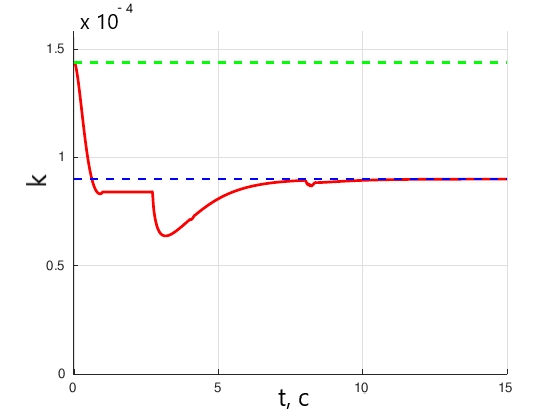
\includegraphics[clip,width=0.44\columnwidth]{k}%
	}
	\quad
	\subfloat[Оценка аэродинамического коэффициента пропеллера $b$]{%
		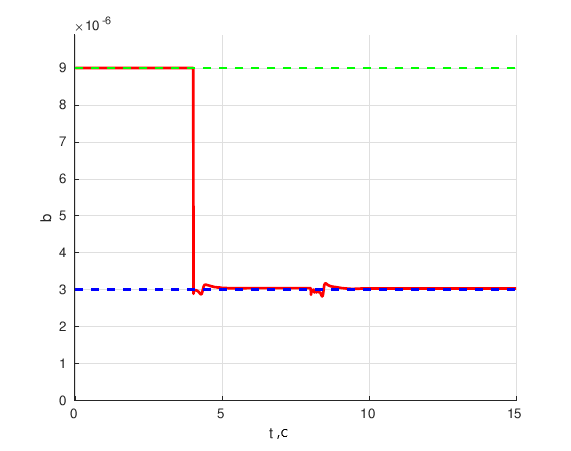
\includegraphics[clip,width=0.44\columnwidth]{b}%
	}
	\caption{ -- Уточнение параметров динамики БЛА}
	\label{fig:observer_k_b}
\end{figure}
\begin{table}[ht]
	\centering
	\caption{ -- Известные параметры модели}\label{tb:observer_params} 
	\begin{tabular}{lcl}
		\hline
		Параметр & Обозначение & Значение  \\\hline
		Общая масса & $M$ & 3,6 кг  \\
		Тензор инерции корпуса & $\bm J_B$ & $diag(53, 63, 98) \cdot{10^{-3}}$ кг$\cdot$м$^2$  \\
		Тензор инерции ротора & $\bm J_R$ & $diag(85, 85, 46) \cdot{10^{-6}}$ кг$\cdot$м$^2$  \\
		Миделево сечение корпуса & $S_{\perp}$ & 0,2 м$^2$ \\
		Луч & $L$ & 0,35 м \\
		Аэродинамический коэффициент & $C$ & 1,05\\	
		Максимальные обороты & $\tilde \omega_{max}$ & 500 рад/с \\		
		Максимальный угол & $\theta_{max}$ & ${\pi}/{4}$ рад \\
		\hline
	\end{tabular}
\end{table}
